\documentclass[tikz]{standalone}
\usepackage{pgfplots}
\pgfplotsset{compat=1.15}
\usepackage{mathrsfs}
\usetikzlibrary{arrows,calc}
\usepackage{tkz-euclide}

\pagestyle{empty}

\definecolor{AngleClr}{rgb}{0,0.39215686274509803,0}
\definecolor{ShapeClr}{rgb}{0.6,0.2,0}

\begin{document}

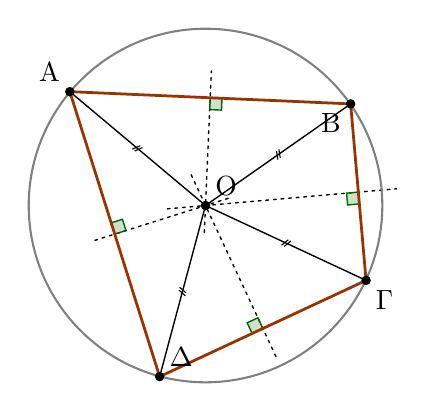
\begin{tikzpicture}[scale=.75]
\tkzSetUpLine[line width=1pt,color=black]
\tkzSetUpPoint[fill=black]

\tkzDefPoint(140:3){A}
\tkzDefPoint(-105:3){D}
\tkzDefPoint(-25:3){C}
\tkzDefPoint(35:3){B}

\tkzDefMidPoint(A,B) \tkzGetPoint{M1}
\tkzDefMidPoint(B,C) \tkzGetPoint{M2}
\tkzDefMidPoint(C,D) \tkzGetPoint{M3}
\tkzDefMidPoint(D,A) \tkzGetPoint{M4}

\tkzDefTriangleCenter[circum](A,B,C) \tkzGetPoint{O}

\tkzFillPolygon[fill=white](A,B,C,D)

\tkzDrawSegments[line width=0.5pt,color=black,dashed,dash pattern=on 1pt off 1.75pt,add=0.25 and 0.25](O,M1 O,M2 O,M3 O,M4)

\tkzMarkRightAngles[line width=0.5pt, size=.2,color=AngleClr,fill=AngleClr,fill opacity=0.2](O,M1,B O,M2,C O,M3,D O,M4,A)

\tkzDrawSegments[line width=0.5pt,color=black](O,A O,B O,C O,D)

\tkzDrawCircle[line width=0.75](O,A)

\tkzDrawPolygon[color=ShapeClr](A,B,C,D)

\tkzDrawPoints[size=3](A,B,C,D, O)
\tkzLabelPoint[above left](A){$\rm A$}
\tkzLabelPoint[below left](B){$\rm B$}
\tkzLabelPoint[below right](C){$\rm \Gamma$}
\tkzLabelPoint[above right](D){$\rm \Delta$}
\tkzLabelPoint[above right](O){$\rm O$}

\tkzMarkSegments[mark=s||,size=1.4](O,A O,B O,C O,D)

\end{tikzpicture}

\end{document}
